\documentclass[11pt]{article}
\usepackage{lipsum}
\usepackage{neurodata}
%===============================================================================%
% This is the project specific preamble for the ND-latex-template.
%
% If you need a specific package please load it here.
% You can either put an `%===============================================================================%
% This is the project specific preamble for the ND-latex-template.
%
% If you need a specific package please load it here.
% You can either put an `%===============================================================================%
% This is the project specific preamble for the ND-latex-template.
%
% If you need a specific package please load it here.
% You can either put an `\input{preamble.tex}` before or after the
% `\usepackage{neurodata}` and deal with any clashes yourself.
% It is important to know which packages clash with our base
% requirements. Thank you
%===============================================================================%


\usepackage{lipsum}
` before or after the
% `\usepackage{neurodata}` and deal with any clashes yourself.
% It is important to know which packages clash with our base
% requirements. Thank you
%===============================================================================%


\usepackage{lipsum}
` before or after the
% `\usepackage{neurodata}` and deal with any clashes yourself.
% It is important to know which packages clash with our base
% requirements. Thank you
%===============================================================================%


\usepackage{lipsum}


\begin{document}

\title{Catchy title here}

\author{}

\maketitle
\thispagestyle{empty}

\noindent
\setcounter{tocdepth}{3}
\setcounter{secnumdepth}{1}

\vspace{-15pt}


\pagenumbering{arabic}
\setcounter{page}{1}

\lipsum[1-3]

\begin{figure}[!h]
    \centering
        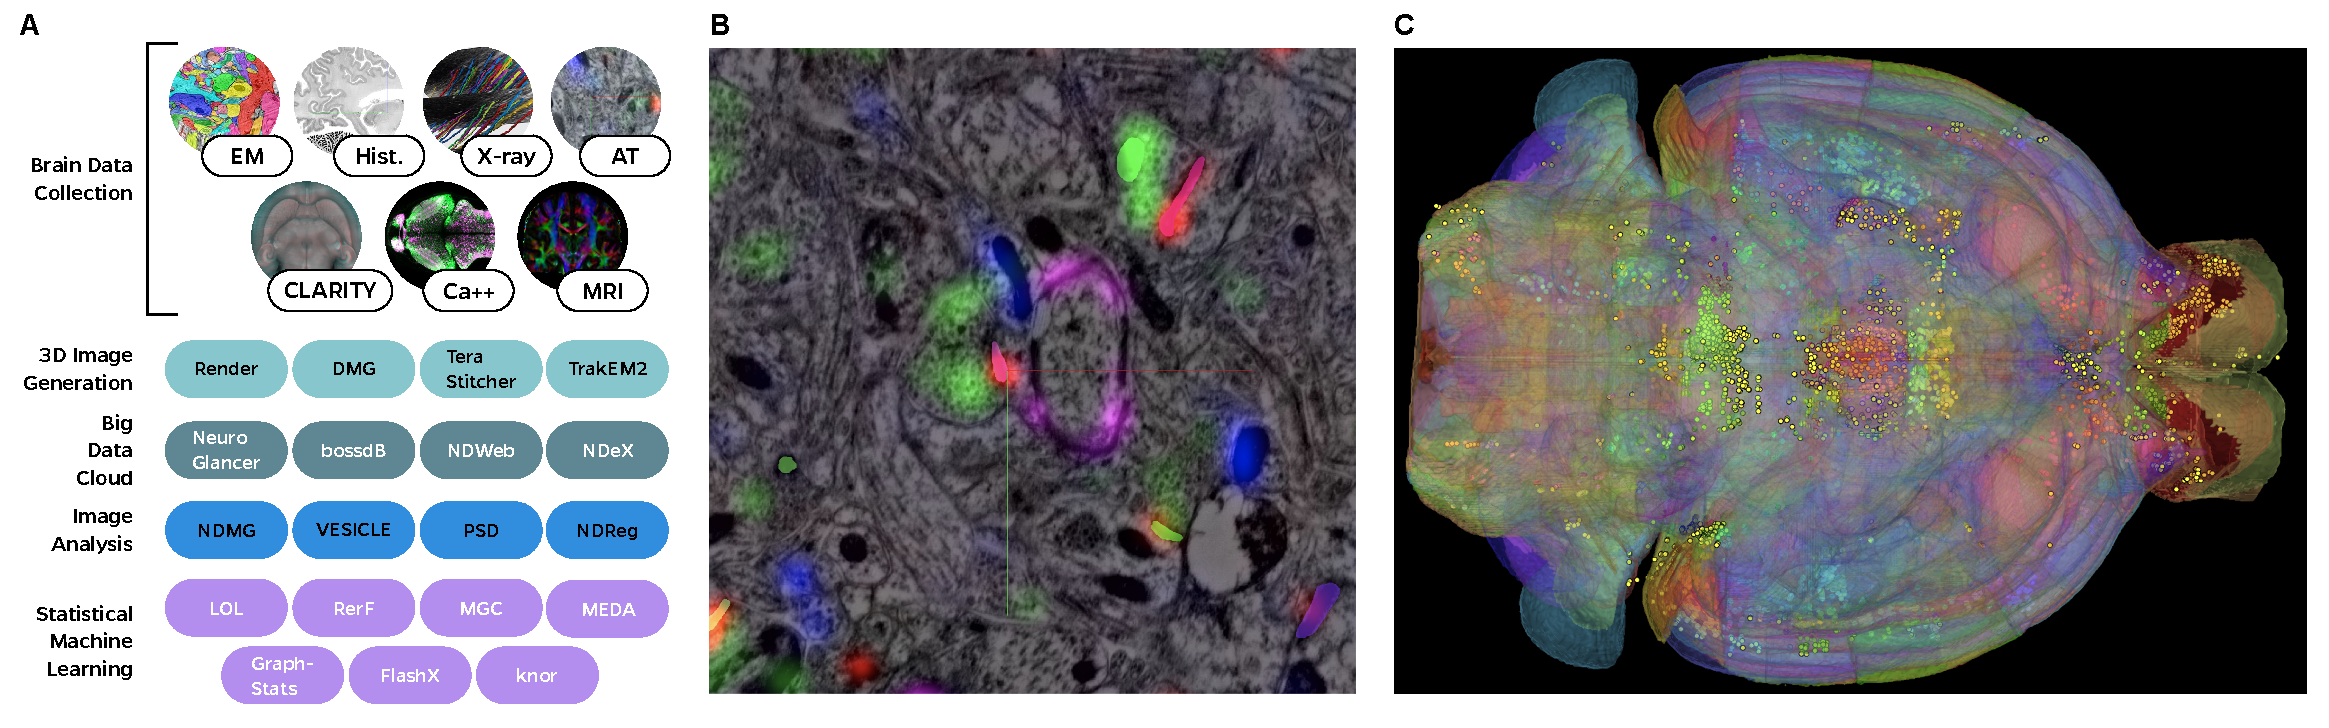
\includegraphics[width=1.0\textwidth]{figs/nd_pipeline_v21.pdf}
    \caption{
  \textbf{(A)}    NeuroData's open-source software ecosystem. 
    }
    \label{fig:1}
\end{figure}

\lipsum[3-5]



% \clearpage 
\paragraph{Data and Code Availability Statement}

\begin{itemize}
    \item All code is available from \url{https://neurodata.io/tools/} under an Apache 2.0 license unless otherwise specified.
	\item All publicly available data is accessible at \url{https://neurodata.io/data/} under the ODC-By v1.0 license, unless otherwise specified.
    \item Figure 1 has images of nearly raw data
\end{itemize}


\paragraph{Authors,  Affiliations, and Acknowledgements}

\nocite{*}

%\section*{References}
\vspace{5mm}
\bibliography{neurodata}
\bibliographystyle{IEEEtran}


\end{document}
